\documentclass[12pt,a4paper]{report}

% ============================================================
% PACKAGES
% ============================================================
\usepackage[utf8]{inputenc}
\usepackage[T1]{fontenc}
\usepackage{graphicx}
\usepackage[margin=1in]{geometry}
\usepackage{fancyhdr}
\usepackage{titlesec}
\usepackage{booktabs}
\usepackage{tabularx}
\usepackage{hyperref}
\usepackage{setspace}
\usepackage{parskip}        % Proper paragraph spacing without indentation issues
\usepackage{enumitem}       % Better list control
\usepackage{array}          % Extended column types in tables
\usepackage{xcolor}         % Color support
\usepackage{listings}       % Code listings
\usepackage{caption}        % Caption control for listings
\usepackage[expansion=false]{microtype}
\usepackage{pdfpages}

% ============================================================
% CODE LISTING STYLE
% ============================================================
\definecolor{codebg}{RGB}{248,248,248}
\definecolor{codeframe}{RGB}{220,220,220}
\definecolor{kwcolor}{RGB}{0,100,180}
\definecolor{strcolor}{RGB}{163,21,21}
\definecolor{cmtcolor}{RGB}{80,120,80}
\definecolor{numcolor}{RGB}{128,0,128}

\lstset{
    language=Python,
    basicstyle=\ttfamily\small,
    keywordstyle=\color{kwcolor}\bfseries,
    stringstyle=\color{strcolor},
    commentstyle=\color{cmtcolor}\itshape,
    numberstyle=\tiny\color{numcolor},
    backgroundcolor=\color{codebg},
    frame=single,
    rulecolor=\color{codeframe},
    numbers=left,
    numbersep=8pt,
    stepnumber=1,
    breaklines=true,
    breakatwhitespace=false,
    showstringspaces=false,
    tabsize=4,
    captionpos=b,
    xleftmargin=1.5em,
    xrightmargin=0.5em,
    aboveskip=10pt,
    belowskip=6pt,
    morekeywords={self, True, False, None, async, await, Optional, Literal},
}

% JavaScript / JSX listing style
\lstdefinelanguage{JavaScript}{
    keywords={const, let, var, function, return, if, else, try, catch, async, await,
               import, export, default, from, class, new, this, typeof, throw,
               require, module, true, false, null, undefined, of, in, for},
    keywordstyle=\color{kwcolor}\bfseries,
    stringstyle=\color{strcolor},
    commentstyle=\color{cmtcolor}\itshape,
    morestring=[b]',
    morestring=[b]",
    morestring=[b]`,
    morecomment=[l]{//},
    morecomment=[s]{/*}{*/},
    sensitive=true,
}

% ============================================================
% HYPERREF CONFIGURATION
% ============================================================
\hypersetup{
    colorlinks=true,
    linkcolor=black,
    citecolor=black,
    urlcolor=black,
    pdftitle={ToneForge: Distributed AI System for Email Formalization, Multi-Agent Negotiation, and Legal Parsing},
    pdfauthor={Arup Mishra, Devayush Kar, Kush Singh, Shreya Banerjee},
}

% ============================================================
% HEADER AND FOOTER
% ============================================================
\pagestyle{fancy}
\fancyhf{}
\fancyfoot[L]{\small School of Computer Engineering, KIIT, Bhubaneswar}
\fancyfoot[R]{\thepage}
\renewcommand{\headrulewidth}{0pt}
\renewcommand{\footrulewidth}{0.4pt}

\fancypagestyle{plagiarism}{
	\fancyhf{}
	\fancyfoot[R]{\thepage}
	\renewcommand{\headrulewidth}{0pt}
	\renewcommand{\footrulewidth}{0pt}
}

% ============================================================
% CHAPTER AND SECTION TITLE FORMATTING
% ============================================================
\titleformat{\chapter}[display]
  {\normalfont\huge\bfseries}{\chaptertitlename\ \thechapter}{20pt}{\Huge}
\titlespacing*{\chapter}{0pt}{-50pt}{40pt}

\titleformat{\section}{\normalfont\Large\bfseries}{\thesection}{1em}{}
\titleformat{\subsection}{\normalfont\large\bfseries}{\thesubsection}{1em}{}

% ============================================================
% LIST FORMATTING
% ============================================================
\setlist[itemize]{noitemsep, topsep=4pt, leftmargin=*}
\setlist[enumerate]{noitemsep, topsep=4pt, leftmargin=*}

% ============================================================
% DOCUMENT BEGIN
% ============================================================
\begin{document}
\onehalfspacing

% ============================================================
% TITLE PAGE
% ============================================================
\begin{titlepage}
	\begin{singlespace}
		\centering
		\vspace*{0.2cm}

		{\Large \textbf{A MINI PROJECT REPORT}}\\[0.4cm]
		{\large on}\\[0.4cm]
		{\LARGE \textbf{``ToneForge: Distributed AI System for Email Formalization,\\[0.2cm] Multi-Agent Negotiation, and Legal Parsing''}}\\[0.8cm]

		{\large Submitted to}\\[0.4cm]
		{\Large \textbf{KIIT Deemed to be University}}\\[0.8cm]

		{\large In Partial Fulfillment of the Requirements for the Award of the}\\[0.4cm]
		{\Large \textbf{BACHELOR OF TECHNOLOGY DEGREE}}\\[0.8cm]

		{\large BY}\\[0.6cm]

		\begin{table}[ht]
			\centering
			\large
			\renewcommand{\arraystretch}{1.4}
			\begin{tabular}{ll@{\hspace{1.8cm}}ll}
				\textbf{Arup Mishra}     & \textbf{23052229} &
				\textbf{Devayush Kar}    & \textbf{23052239}   \\
				\textbf{Kush Singh}      & \textbf{23052247} &
				\textbf{Shreya Banerjee} & \textbf{23052267}   \\
			\end{tabular}
		\end{table}

		\vfill

		{\large UNDER THE GUIDANCE OF}\\[0.4cm]
		{\Large \textbf{Dr.\ Ajit Kumar Pasayat}}\\
		{\large Associate Professor, School of Computer Engineering}\\[0.8cm]

		
\includegraphics[width=0.35\textwidth]{img/kiit_logo.png}

		\vfill

		{\large \textbf{SCHOOL OF COMPUTER ENGINEERING}}\\
		{\large \textbf{KALINGA INSTITUTE OF INDUSTRIAL TECHNOLOGY}}\\
		{\large \textbf{(Deemed to be University)}}\\
		{\large \textbf{BHUBANESWAR, ODISHA - 751024}}\\[0.4cm]
		{\large \textbf{March 2026}}
	\end{singlespace}
\end{titlepage}

% ============================================================
% FRONT MATTER
% ============================================================
\pagenumbering{roman}

% ------------------------------------------------------------
% CERTIFICATE
% ------------------------------------------------------------
\chapter*{CERTIFICATE}
\addcontentsline{toc}{chapter}{Certificate}

This is to certify that the project entitled \textbf{``ToneForge: Distributed AI System for Email Formalization, Multi-Agent Negotiation, and Legal Parsing''} submitted by \textbf{Arup Mishra (23052229), Devayush Kar (23052239), Kush Singh (23052247), and Shreya Banerjee (23052267)} is a record of bona fide work carried out by them in partial fulfillment of the requirements for the award of the Degree of Bachelor of Technology in Computer Science and Engineering at KIIT Deemed to be University, Bhubaneswar.

This work was carried out during the Academic Year 2025-26 (6th Semester) under my guidance and supervision. To the best of my knowledge, the work presented here has not been submitted elsewhere, either in part or full, for the award of any degree or diploma.

\vspace{3cm}

\noindent
\begin{tabular*}{\textwidth}{@{\extracolsep{\fill}}lr}
	Place: Bhubaneswar & \rule{6cm}{0.4pt} \\
	Date: \rule{3cm}{0.4pt} & \textbf{Dr.\ Ajit Kumar Pasayat} \\
	& Associate Professor \\
	& School of Computer Engineering, KIIT \\
\end{tabular*}

\clearpage

% ------------------------------------------------------------
% ACKNOWLEDGEMENTS
% ------------------------------------------------------------
\chapter*{Acknowledgements}
\addcontentsline{toc}{chapter}{Acknowledgements}

We would like to express our sincere gratitude to \textbf{Dr.\ Ajit Kumar Pasayat}, Associate Professor, School of Computer Engineering, KIIT University, for his expert guidance, unwavering encouragement, and constructive feedback throughout the duration of this project, from its inception to completion.

We are also grateful to the faculty and staff of the School of Computer Engineering, KIIT, for providing the academic environment and resources necessary for this work. Finally, we extend our thanks to our families and peers for their continued support and motivation.

\vspace{2.5cm}

\noindent \textbf{Signatures:}

\vspace{1.5cm}
\noindent
\begin{tabular*}{\textwidth}{@{\extracolsep{\fill}}lr}
	\rule{5.5cm}{0.4pt} & \rule{5.5cm}{0.4pt} \\
	Arup Mishra (23052229) & Devayush Kar (23052239) \\
	\\[1.5cm]
	\rule{5.5cm}{0.4pt} & \rule{5.5cm}{0.4pt} \\
	Kush Singh (23052247) & Shreya Banerjee (23052267) \\
\end{tabular*}

\clearpage

% ------------------------------------------------------------
% ABSTRACT
% ------------------------------------------------------------
\chapter*{Abstract}
\addcontentsline{toc}{chapter}{Abstract}

ToneForge is a distributed web application designed to automate and enhance professional communication using Large Language Models (LLMs). The system architecture comprises three discrete tiers: a React-based frontend for user interaction, a Node.js/Express API gateway responsible for authentication and data persistence via MongoDB, and an isolated Python microservice built on FastAPI that orchestrates heavy AI computation.

The platform delivers three primary natural language processing capabilities: (i) contextual email formalization and multi-lingual translation across predefined professional registers (business, academic, and corporate); (ii) structural parsing of legal correspondence to extract obligations, deadlines, and risk classifications; and (iii) multi-agent negotiation simulation coordinated through LangGraph, wherein specialized LLM agents (Proposer, Responder, and Evaluator) iteratively converge on a draft agreement. The Groq inference API provides low-latency LLM execution via the \texttt{openai/gpt-oss-120b} model, while Pydantic schemas enforce strict data validation at the service boundary.

ToneForge demonstrates the effective integration of conventional full-stack web paradigms with stateful AI orchestration frameworks, providing a scalable and extensible foundation for enterprise-grade communication tooling.

\vspace{1cm}
\noindent \textbf{Keywords:} Microservice Architecture, LangGraph, Multi-Agent Negotiation, Natural Language Processing, MERN Stack, FastAPI, Groq API.

\clearpage

% ------------------------------------------------------------
% TABLE OF CONTENTS, FIGURES, TABLES
% ------------------------------------------------------------
\tableofcontents
\clearpage
\listoffigures
\clearpage
\listoftables
\clearpage

% ============================================================
% MAIN CONTENT
% ============================================================
\pagenumbering{arabic}

% ============================================================
\chapter{Introduction}
% ============================================================

\section{Project Overview}
ToneForge is a full-stack, AI-driven platform designed to standardize, translate, and analyze professional correspondence. To ensure scalability and clear separation of concerns, the application is structured into two discrete subsystems. The primary web infrastructure employs the MERN stack (MongoDB, Express.js, React, Node.js) to manage user authentication via JSON Web Tokens (JWT), session security, and historical record tracking. In parallel, a dedicated Python microservice, built with FastAPI, LangChain, and LangGraph, handles complex text processing tasks by interfacing with the Groq inference engine to execute LLM workflows.

\section{Motivation and Problem Statement}
Professional email communication demands strict adherence to register, structural norms, and, in many contexts, legal constraints. Non-native English speakers and individuals communicating outside their primary domain frequently encounter difficulty in conforming to these requirements, which can result in miscommunication or unintended legal liability.

While existing software provides basic orthographic correction or short-form reply generation, no widely available tool offers mechanisms for full structural document transformation, automated negotiation simulation, or clause-level risk extraction. The problem therefore necessitates an automated pipeline capable of parsing unstructured natural language, classifying its intent and associated risk parameters, and regenerating it into formally structured output. ToneForge addresses this gap by applying agentic LLM workflows and strict schema enforcement to raw text inputs.

\section{Objectives}
The primary objectives of the ToneForge project are:
\begin{itemize}
	\item To design a distributed architecture that decouples the user-facing web server (Node.js) from the AI execution engine (FastAPI), ensuring independent scalability.
	\item To implement a secure user management system using JSON Web Tokens (JWT) and bcrypt-encrypted credential storage in MongoDB.
	\item To develop a stateful multi-agent negotiation system using LangGraph, simulating iterative dialogue between a Proposer, Responder, and neutral Evaluator agent.
	\item To construct a structured parser capable of extracting obligations, deadlines, and risk ratings from unstructured legal correspondence.
	\item To enforce rigorous data validation across all service boundaries using Pydantic schemas and JSON contracts.
\end{itemize}

\section{Scope of the Project}

\noindent\textbf{In Scope:}
\begin{itemize}
	\item Secure user authentication and per-user generation history tracking.
	\item Text formalization mapped to three predefined professional registers: business, academic, and corporate.
	\item Multi-language translation support integrated directly with the formalization output.
	\item Negotiation loop simulation with deterministic termination conditions (maximum 6 rounds; default 3). Supported registers are \texttt{business} and \texttt{corporate}.
	\item Classification of legal clauses by risk level: Low, Medium, and High.
\end{itemize}

\noindent\textbf{Out of Scope:}
\begin{itemize}
	\item Direct integration with email client protocols (IMAP/SMTP).
	\item Fine-tuning of base LLM weights; the system relies entirely on prompt engineering and in-context learning.
	\item Parsing of binary file attachments such as PDFs or Word documents.
\end{itemize}

\section{Implementation Summary}
The core AI orchestration is powered by LangGraph, which enables stateful, multi-step LLM workflows. Unlike traditional linear chains, the implementation utilizes cyclic graph structures to analyze, formalize, and translate correspondence. This ensures that the system can short-circuit processes if an email is already formal or dynamically route text to specialized expert nodes based on the detected category. Furthermore, agentic features facilitate multi-party negotiation simulations and structured legal risk extraction through iterative LLM reasoning cycles.

% ============================================================
\chapter{Literature Survey}
% ============================================================

\section{Existing Systems and Comparative Analysis}
The domain of automated text generation has expanded considerably since the introduction of transformer-based language models. The following table benchmarks ToneForge against existing tools with respect to specific functional capabilities relevant to professional communication, rather than general-purpose chatbot utility.

\begin{table}[ht]
	\centering
	\renewcommand{\arraystretch}{1.6}
	\setlength{\tabcolsep}{8pt}
	\begin{tabularx}{\textwidth}{>{\raggedright}p{2.8cm} >{\raggedright}p{2.8cm} >{\raggedright}p{2.4cm} >{\raggedright}p{2.6cm} >{\raggedright\arraybackslash}X}
		\toprule
		\textbf{System}    & \textbf{Email Formalization}     & \textbf{Data Persistence} & \textbf{Agentic Negotiation}   & \textbf{Legal Parsing}   \\
		\midrule
		Grammarly          & Partial (tone only)              & No                        & No                             & No                       \\
		Gmail Smart Reply  & Short-form only                  & Yes                       & No                             & No                       \\
		ChatGPT (Standard) & Manual prompting                 & Session-level             & Manual prompting               & Unstructured             \\
		\textbf{ToneForge} & \textbf{Parameterized registers} & \textbf{Secure (MongoDB)} & \textbf{Automated (LangGraph)} & \textbf{Structured JSON} \\
		\bottomrule
	\end{tabularx}
	\caption{Functional Capabilities Comparison with Existing Systems}
\end{table}

\section{Research Gap and System Novelty}
ToneForge draws from foundational research in the LangChain ecosystem \cite{chase} and generative multi-agent simulation \cite{park}, integrating these paradigms into a cohesive, production-oriented web application. The primary areas of novelty are:

\begin{itemize}
	\item \textbf{Isolated Agentic Loops:} Unlike standard linear API call chains, the negotiation feature employs a cyclic directed graph (via LangGraph). The Proposer and Responder agents iterate asynchronously until the Evaluator agent signals convergence or the predefined depth limit is reached.
	\item \textbf{Structured Extraction:} The legal parser transforms inherently unstructured informal correspondence into rigid, queryable data structures enforced by Pydantic schemas. This enables frontend applications to render rich dashboards displaying risk flags, obligations, and deadline summaries.
	\item \textbf{Distributed Component Integration:} The project demonstrates how standard full-stack authentication paradigms can be cleanly bridged with stateless, high-latency AI microservices through a proxy gateway pattern.
\end{itemize}

% ============================================================
\chapter{Requirement Specifications and System Design}
% ============================================================

\section{Software Requirements Specification}

\subsection{Functional Requirements}
\begin{itemize}
	\item \textbf{FR-01:} The system shall require user authentication via JWT to access all AI generation endpoints.
	\item \textbf{FR-02:} The Node.js gateway shall persist all user queries and AI responses to a MongoDB \texttt{History} collection.
	\item \textbf{FR-03:} The formalization endpoint shall transform input text based on a caller-specified register and target language parameter.
	\item \textbf{FR-04:} The legal parsing endpoint shall return a validated JSON payload strictly defining obligations, clauses, and risk categorizations.
	\item \textbf{FR-05:} The \texttt{/negotiate\_email} endpoint shall orchestrate multiple asynchronous LLM calls via LangGraph across Proposer, Responder, and Evaluator nodes (supporting \texttt{business} and \texttt{corporate} categories), returning the full conversational thread and a final summary upon convergence or timeout.
\end{itemize}

\subsection{Non-Functional Requirements}
\begin{itemize}
	\item \textbf{NFR-01 (Latency):} Inter-service communication via Axios must be non-blocking at the gateway level to avoid degrading concurrent user sessions during long-running AI calls.
	\item \textbf{NFR-02 (Security):} User passwords shall be hashed using BcryptJS prior to storage. Groq API keys shall be confined strictly to server-side environment variables and must never be transmitted to or accessible by the client.
	\item \textbf{NFR-03 (Reliability):} The FastAPI microservice shall handle upstream inference errors (e.g., rate limits, malformed LLM outputs) and return standardized HTTP error codes with descriptive messages to the Node.js gateway.
\end{itemize}

\section{Hardware and Software Requirements}

\textbf{Hardware Requirements (Development Environment):}
\begin{itemize}
	\item \textbf{Processor:} Intel Core i5 / AMD Ryzen 5 or higher.
	\item \textbf{RAM:} 8 GB minimum (16 GB recommended for running dual servers and compilation).
	\item \textbf{Storage:} 256 GB SSD or higher.
	\item \textbf{Network:} Stable broadband connection for Groq LPU API inference and MongoDB Atlas access.
\end{itemize}

\textbf{Software Requirements:}
\begin{itemize}
	\item \textbf{Operating System:} Windows 10/11, macOS, or Linux (Ubuntu 20.04+).
	\item \textbf{Runtime Environments:} Node.js (v18.x or higher) and Python (v3.11 or higher).
	\item \textbf{Frontend Dependencies:} React (v19.2.0), Vite (v7.3.1), TailwindCSS (v4.1.18), Framer Motion (v12.34.3), React Router DOM (v7.13.0).
	\item \textbf{Backend Dependencies:} Express.js (v4.18.0), Mongoose (v9.2.1), JSONWebToken (v9.0.3), BcryptJS (v3.0.3).
	\item \textbf{Microservice Dependencies:} FastAPI, Uvicorn, LangChain-Groq, LangGraph, Pydantic, Python-Dotenv.
	\item \textbf{Database:} MongoDB Atlas (Cloud deployment).
\end{itemize}

\section{System Architecture}
ToneForge operates on a three-tier distributed architecture that segregates client interaction, user management, and AI computation into independent layers.

\begin{figure}[ht]
	\centering
	% Ensure architecture.png is in the same folder as this .tex file
	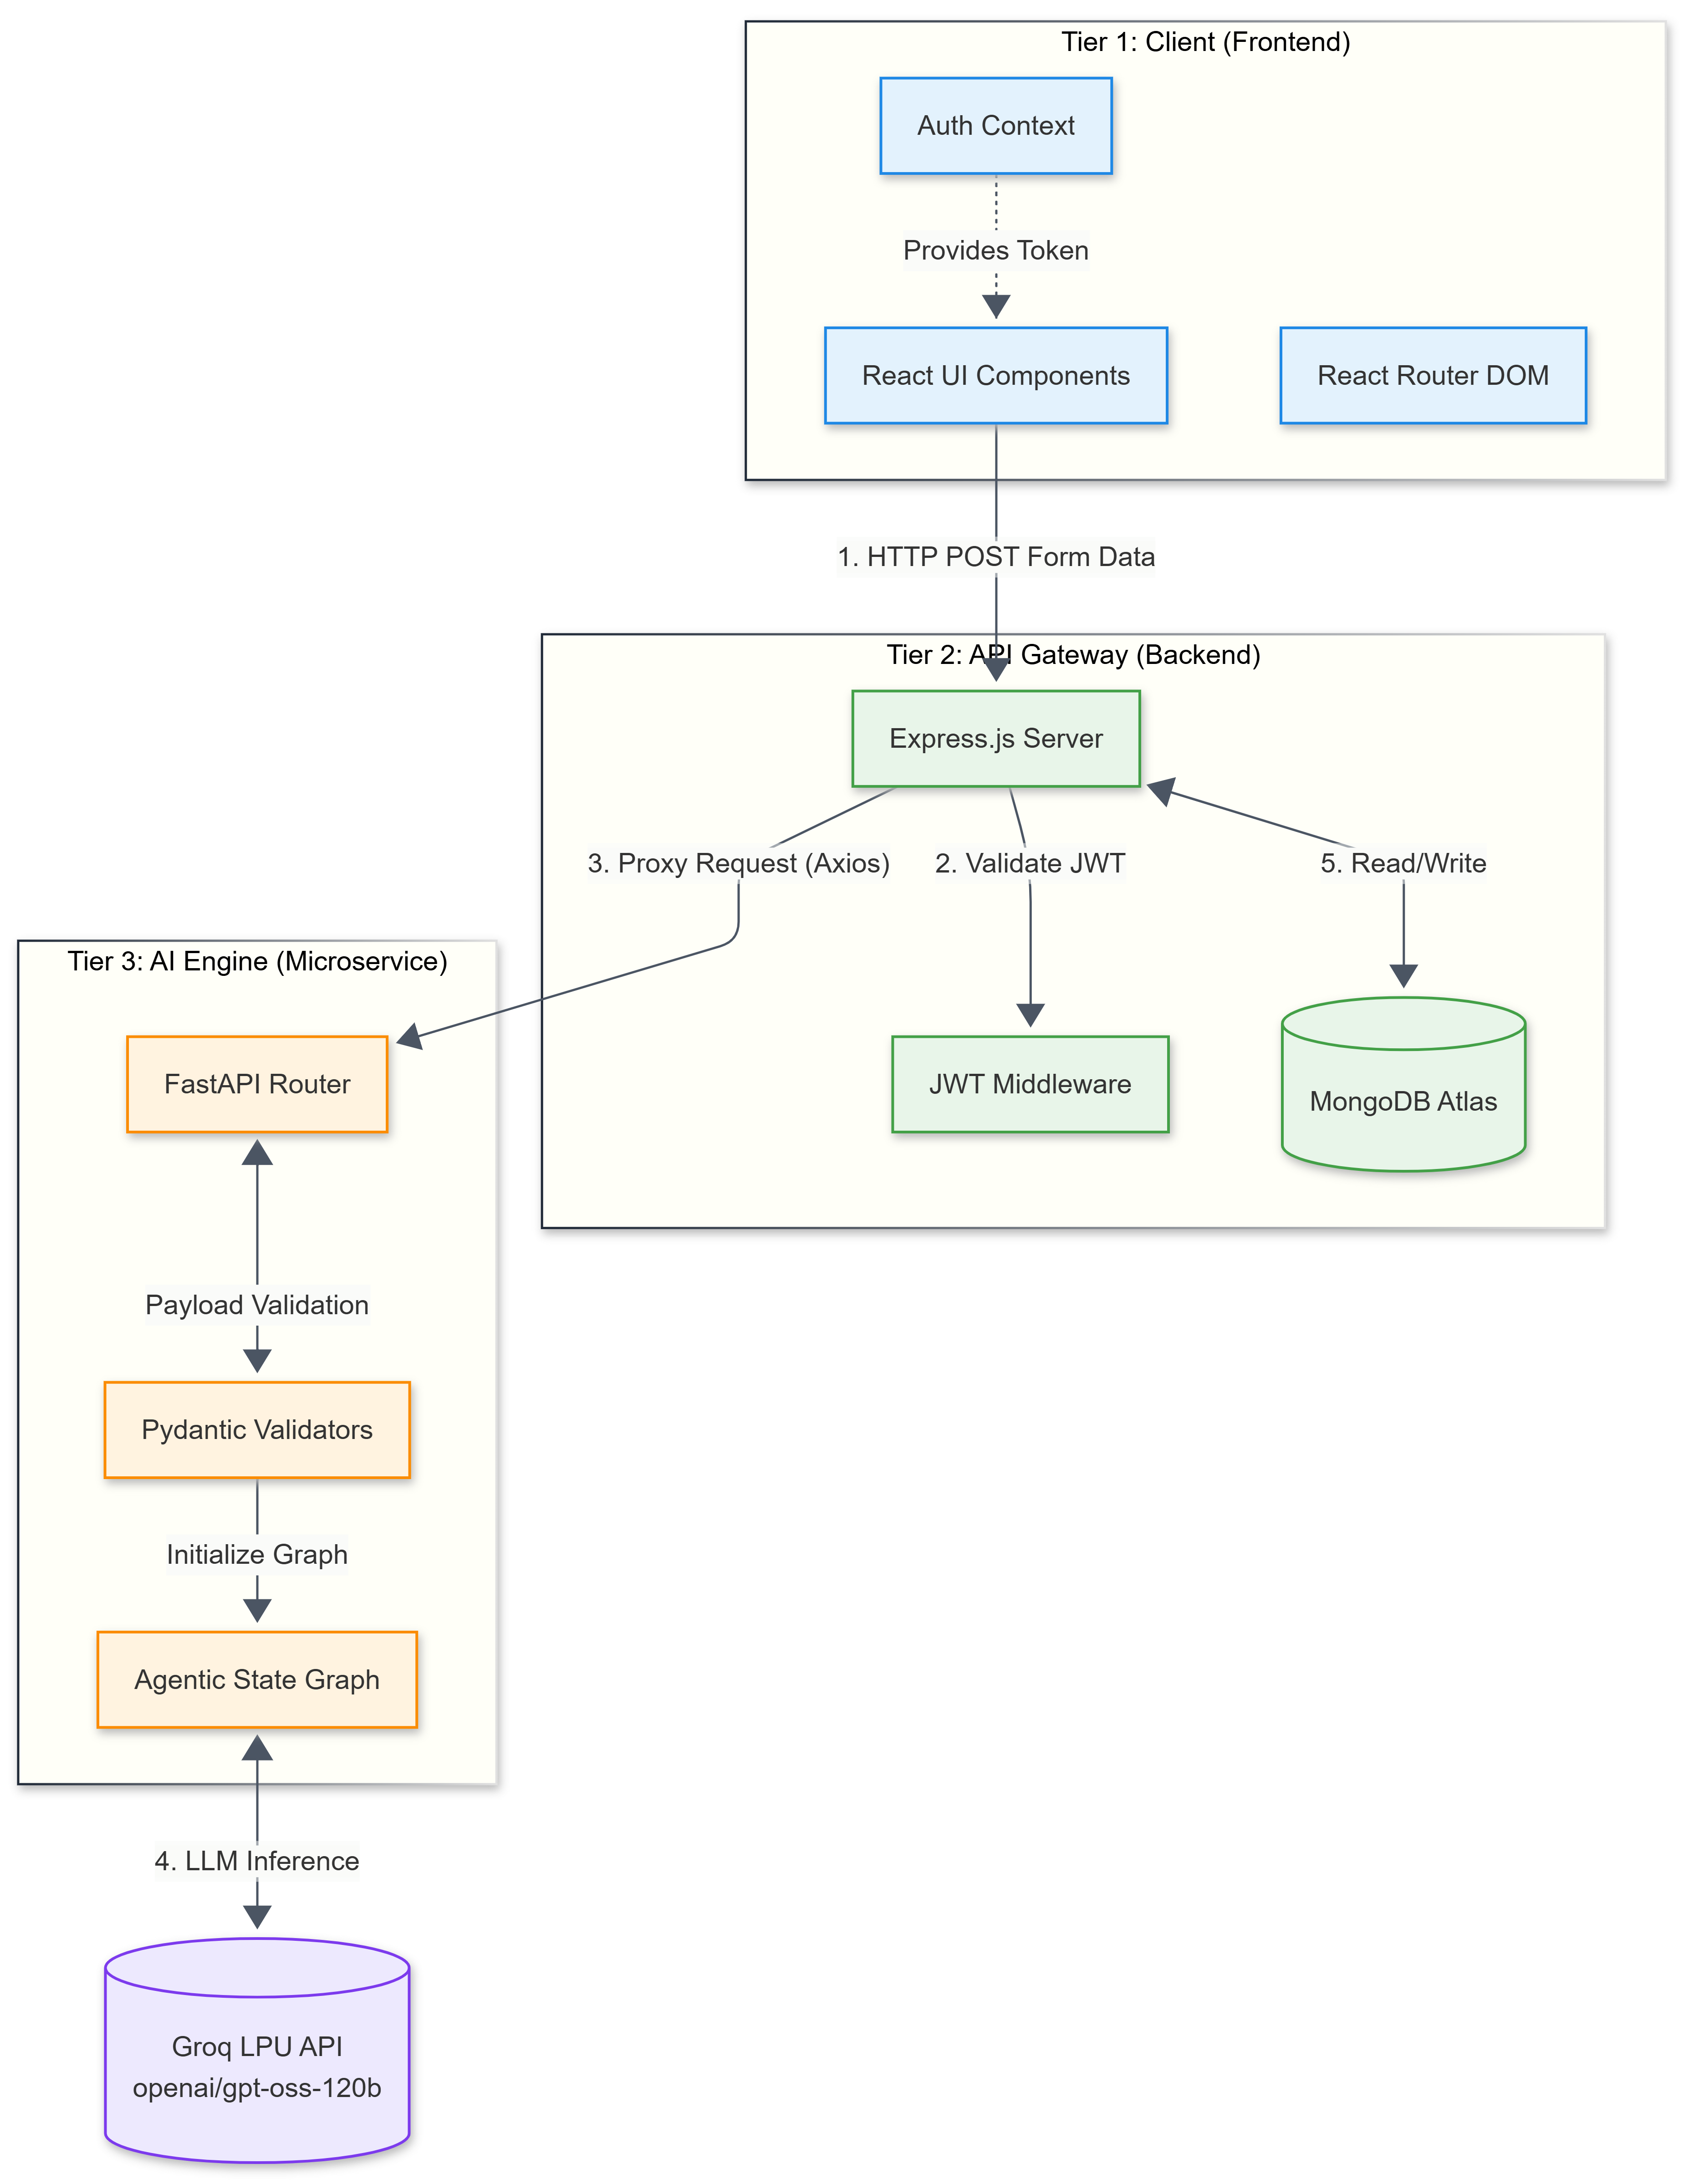
\includegraphics[width=0.9\textwidth]{img/architecture.png}
	\caption{ToneForge System Architecture Flow}
	\label{fig:architecture}
\end{figure}

\begin{table}[ht]
	\centering
	\renewcommand{\arraystretch}{1.4}
	\begin{tabularx}{\textwidth}{lX}
		\toprule
		\textbf{Layer}           & \textbf{Technology and Responsibility}                                                                                                                                                  \\
		\midrule
		Client (Frontend)        & \textbf{React 19 (Vite), TailwindCSS, Framer Motion.} Manages UI state, client-side routing, and submission of form payloads to the API Gateway.                                        \\
		API Gateway (Backend)    & \textbf{Node.js, Express, MongoDB.} Handles routes (\texttt{/api/auth}, \texttt{/api/history}). Verifies JWTs, persists history, and proxies validated requests to the AI microservice. \\
		AI Engine (Microservice) & \textbf{Python 3.11, FastAPI, LangGraph, Groq.} Receives validated text payloads, executes prompt chains and graph iterations, and returns schema-compliant JSON responses.             \\
		\bottomrule
	\end{tabularx}
	\caption{Three-Tier Distributed Architecture Overview}
\end{table}

\subsection{Data Flow: Negotiation Workflow}
The following sequence describes the end-to-end data flow for the multi-agent negotiation feature:

\begin{figure}[ht]
	\centering
	% Ensure data_flow.png is in the same folder as this .tex file
	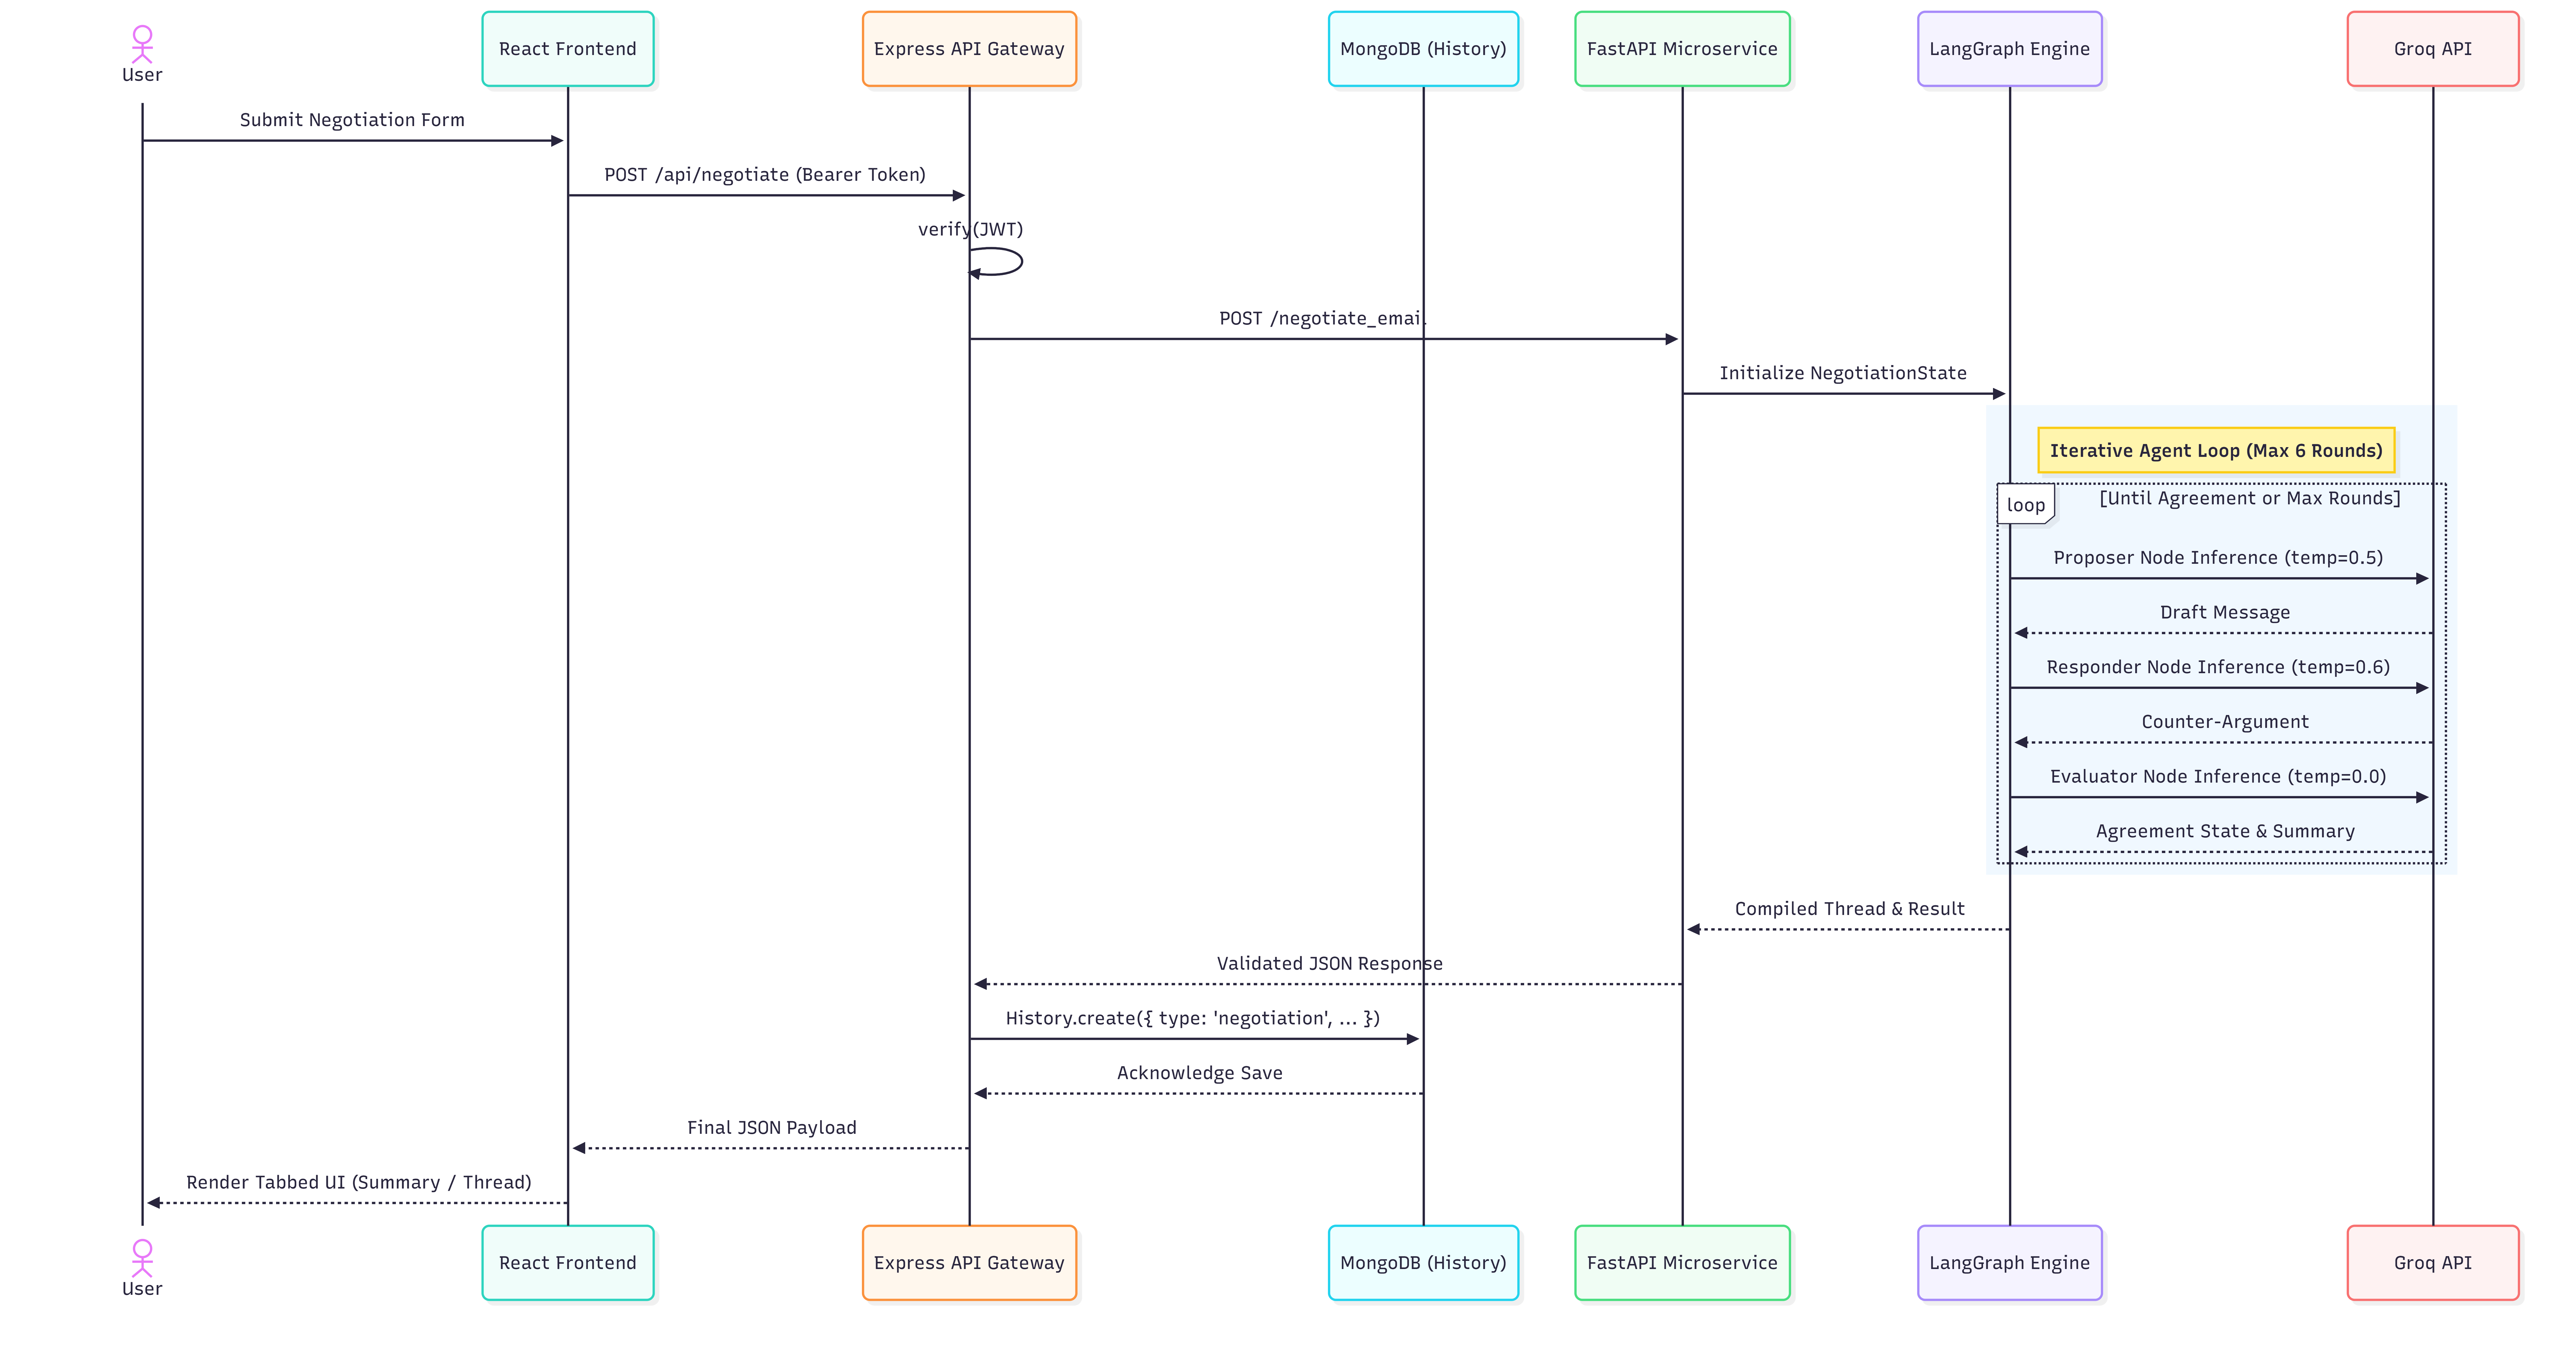
\includegraphics[width=1.0\textwidth]{img/data_flow.png}
	\caption{Sequence Diagram of the Multi-Agent Negotiation Data Flow}
	\label{fig:data_flow}
\end{figure}

\begin{enumerate}
	\item The React client submits initial parameters (\texttt{topic}, \texttt{our\_position}, \texttt{their\_position}) to the Express API gateway.
	\item The gateway authenticates the request via JWT middleware, then forwards the payload via Axios to the FastAPI \texttt{POST /negotiate\_email} endpoint.
	\item LangGraph initializes the negotiation state graph. The \textbf{Proposer} node generates the initial draft message.
	\item The \textbf{Responder} node generates a counter-argument conditioned on \texttt{their\_position}.
	\item The \textbf{Evaluator} node analyzes the current thread and determines whether an agreement has been reached. If so, the cycle terminates; otherwise, control returns to the Proposer for a subsequent round (up to \texttt{max\_rounds}, default 3, maximum 6).
	\item FastAPI returns the compiled negotiation thread and a final summary. The gateway logs the result to MongoDB and forwards the response JSON to the React client.
\end{enumerate}

\subsection{Frontend Page Structure}
The React application defines eight client-side routes via React Router. The public routes (\texttt{/}, \texttt{/login}, and \texttt{/signup}) are accessible without authentication. The remaining five routes (\texttt{/editor}, \texttt{/legal}, \texttt{/negotiate}, \texttt{/history}, and \texttt{/profile}) are each wrapped in a \texttt{ProtectedRoute} component that redirects unauthenticated users to the login page. The following table summarizes the purpose of each protected view.

\begin{table}[ht]
	\centering
	\renewcommand{\arraystretch}{1.4}
	\begin{tabularx}{\textwidth}{lX}
		\toprule
		\textbf{Route}      & \textbf{Page and Responsibility}                                                                                                                                                                                                                 \\
		\midrule
		\texttt{/editor}    & \textbf{EditorPage}: Accepts raw email input, a register selector (Business, Academic, Corporate), and an optional target language. Submits to \texttt{/api/convert} and renders the formalized and optionally translated result.                \\
		\texttt{/legal}     & \textbf{LegalPage}: Accepts legal correspondence text and submits to \texttt{/api/parse\_legal}. Renders an executive summary, an obligation/deadline/risk-flag grid, and a horizontally scrollable clause carousel with per-clause risk badges. \\
		\texttt{/negotiate} & \textbf{NegotiationPage}: Two-column layout with a form for topic, positions, category, and round count on the left, and tabbed results (Summary and Email Thread views) on the right. Submits to \texttt{/api/negotiate}.                       \\
		\texttt{/history}   & \textbf{HistoryPage}: Fetches all past records from \texttt{/api/history} and renders them as typed cards, distinguishing between formalization, legal, and negotiation entries using the \texttt{type} field from the History schema.           \\
		\texttt{/profile}   & \textbf{ProfilePage}: Displays user email, member-since date, and total conversion count retrieved from \texttt{/api/users/profile}.                                                                                                             \\
		\bottomrule
	\end{tabularx}
	\caption{Protected Frontend Routes and Their Responsibilities}
\end{table}

% ============================================================
\chapter{Implementation}
% ============================================================

\section{Technology Stack}
The implementation employs a set of technologies chosen to match the specific requirements of each architectural layer.

\begin{table}[ht]
	\centering
	\renewcommand{\arraystretch}{1.4}
	\begin{tabularx}{\textwidth}{llX}
		\toprule
		\textbf{Component} & \textbf{Technology}     & \textbf{Purpose}                                                                 \\
		\midrule
		Frontend Framework & React.js 19 (Vite)      & Component-based UI construction and client-side routing.                         \\
		API Gateway        & Node.js and Express.js  & RESTful API, request validation, JWT enforcement, and microservice proxying.     \\
		Database           & MongoDB (Mongoose ODM)  & Persistent storage of user profiles and generation history records.              \\
		AI Microservice    & FastAPI (Python 3.11)   & Asynchronous orchestration and serving of LLM workflows.                         \\
		LLM Orchestration  & LangChain and LangGraph & Prompt templating, structured output parsing, and cyclic agent graph execution.  \\
		Inference Provider & Groq API                & Hardware-accelerated LLM inference using the \texttt{openai/gpt-oss-120b} model. \\
		\bottomrule
	\end{tabularx}
	\caption{Detailed Technology Stack}
\end{table}

\section{Key Implementation Details}

\subsection{API Endpoint Surface}
The microservice exposes four \texttt{POST} endpoints, partitioned across two modules. \texttt{core\_features.py} provides \texttt{/formalize\_email}, which rewrites raw input into the requested professional register and optionally translates the result, and \texttt{/generate\_reply}, which produces a tone-matched reply to an incoming email. \texttt{agent\_features.py} provides \texttt{/negotiate\_email}, which orchestrates the multi-agent negotiation graph, and \texttt{/parse\_legal\_email}, which runs structured clause extraction. All four endpoints are mounted on the FastAPI application instance in \texttt{main.py} via \texttt{APIRouter} inclusion.

The request and response contracts for the agentic endpoints are enforced via Pydantic models, as shown in Listing~\ref{lst:schemas}. \texttt{NegotiationRequest} constrains the category to \texttt{business} or \texttt{corporate} and bounds \texttt{max\_rounds} between 1 and 6. \texttt{LegalParseOutput} defines the full structured output, including typed clause objects with an enumerated risk level.

\begin{lstlisting}[caption={Pydantic request and output schemas for the agentic endpoints (\texttt{agent\_features.py})}, label={lst:schemas}]
class NegotiationRequest(BaseModel):
    topic: str
    our_position: str
    their_position: str
    category: Literal["business", "corporate"]
    max_rounds: int = Field(default=3, ge=1, le=6)

class LegalClause(BaseModel):
    clause_type: str   # e.g. Liability, Confidentiality, Payment
    text: str
    risk_level: Literal["low", "medium", "high"]

class LegalParseOutput(BaseModel):
    obligations: list[str]
    deadlines: list[str]
    clauses: list[LegalClause]
    risk_flags: list[str]
    overall_risk: Literal["low", "medium", "high"]
    plain_summary: str
\end{lstlisting}

\subsection{Inter-Service Communication}
The Node.js server acts as a reverse proxy for all AI functionality. Each gateway endpoint follows the same pattern: validate the JWT, forward the request body via \texttt{axios.post} to the Python microservice at \texttt{AI\_BASE\_URL}, save the result to MongoDB, and return the response to the client. Listing~\ref{lst:proxy} shows this pattern for the \texttt{/api/negotiate} endpoint.

\begin{lstlisting}[language=JavaScript, caption={Gateway proxy pattern: JWT-protected route forwarding to the AI microservice and saving to MongoDB (\texttt{server/index.js})}, label={lst:proxy}]
app.post('/api/negotiate', protect, async (req, res) => {
  const { topic, our_position, their_position, category, max_rounds } = req.body;
  const finalMaxRounds = Math.min(Math.max(parseInt(max_rounds) || 3, 1), 6);

  const response = await axios.post(`${AI_BASE_URL}/negotiate_email`, {
    topic, our_position, their_position,
    category: category || 'business',
    max_rounds: finalMaxRounds
  }, { headers: { 'Authorization': `Bearer ${AI_API_KEY}` } });

  const aiResult = response.data;

  // Persist to MongoDB History collection
  await History.create({
    userId: req.user.id,
    type: 'negotiation',
    topic: aiResult.topic || topic,
    roundsCompleted: aiResult.rounds_completed,
    agreementReached: aiResult.agreement_reached,
    summary: aiResult.summary,
    emailThread: aiResult.email_thread
  });

  res.json(aiResult);
});
\end{lstlisting}

\subsection{JWT Authentication Middleware}
The \texttt{protect} middleware in \texttt{authMiddleware.js} guards all non-public routes. It extracts the Bearer token from the \texttt{Authorization} header, verifies it against \texttt{JWT\_SECRET}, and resolves the associated user from MongoDB. Distinct error responses are returned for the three failure cases: missing token, expired token (\texttt{TokenExpiredError}), and malformed token (\texttt{JsonWebTokenError}).

\begin{lstlisting}[language=JavaScript, caption={JWT authentication middleware with differentiated error handling (\texttt{server/middleware/authMiddleware.js})}, label={lst:auth}]
const protect = async (req, res, next) => {
    let token;
    if (req.headers.authorization?.startsWith('Bearer')) {
        try {
            token = req.headers.authorization.split(' ')[1]?.trim();
            const decoded = jwt.verify(token, process.env.JWT_SECRET);
            req.user = await User.findById(decoded.id).select('-password');
            if (!req.user) return res.status(401).json({ error: 'User not found' });
            next();
        } catch (error) {
            if (error.name === 'TokenExpiredError')
                return res.status(401).json({ error: 'Not authorized, token expired' });
            if (error.name === 'JsonWebTokenError')
                return res.status(401).json({ error: 'Not authorized, token invalid' });
            res.status(401).json({ error: 'Not authorized, token failed' });
        }
    }
    if (!token) return res.status(401).json({ error: 'No token provided' });
};
\end{lstlisting}

\subsection{Mongoose Data Schemas}
The \texttt{History} Mongoose schema uses a \texttt{type} discriminator field (\texttt{formalization}, \texttt{legal}, \texttt{negotiation}) to store all three operation types in a single collection. Fields irrelevant to a given type are simply left undefined, leveraging MongoDB's schemaless flexibility while still enforcing field-level types. The \texttt{User} schema implements a bcrypt pre-save hook that hashes the password only when it has been modified, preventing double-hashing on subsequent saves.

\begin{figure}[ht]
	\centering
	% Ensure er_schema.png is in the same folder as this .tex file
	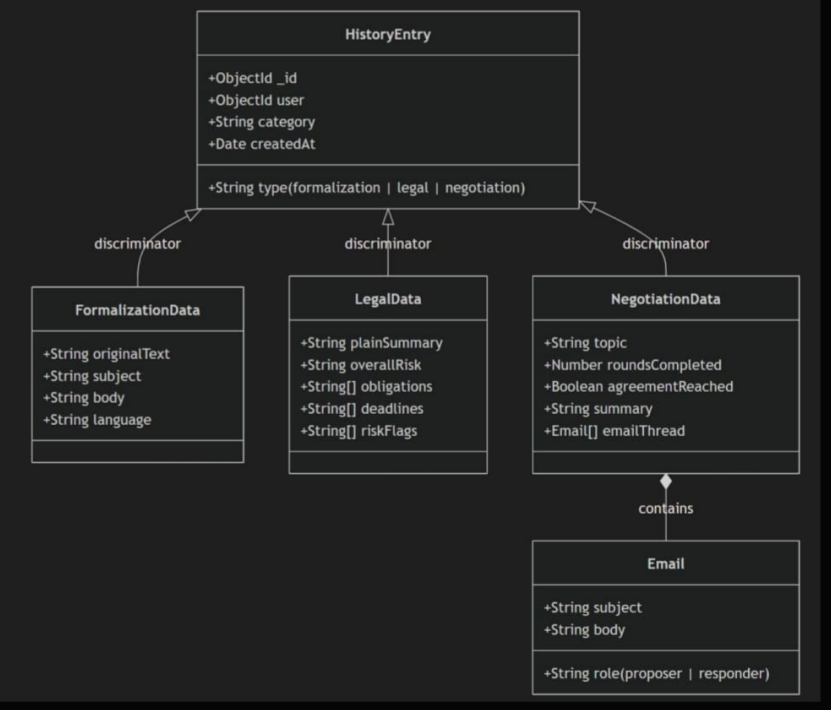
\includegraphics[width=0.8\textwidth]{img/er_schema.png}
	\caption{Entity-Relationship Schema for User and History Collections}
	\label{fig:er_schema}
\end{figure}

\begin{lstlisting}[language=JavaScript, caption={Polymorphic History schema with type discriminator, and User schema with bcrypt pre-save hook (\texttt{server/models/})}, label={lst:schemas_js}]
// History.js - single collection, three operation types
const historySchema = new mongoose.Schema({
    userId:   { type: mongoose.Schema.Types.ObjectId, ref: 'User', required: true },
    type:     { type: String, enum: ['formalization', 'legal', 'negotiation'] },
    originalText: { type: String, required: true },
    // Formalization fields
    formalizedText: String,  subject: String,
    category: { type: String, enum: ['business', 'academic', 'corporate'] },
    language: String,  translatedBody: String,  translatedSubject: String,
    // Legal fields
    obligations: [String],  deadlines: [String],
    clauses: [{ clause_type: String, text: String, risk_level: String }],
    riskFlags: [String],  overallRisk: String,  plainSummary: String,
    // Negotiation fields
    topic: String,  roundsCompleted: Number,
    agreementReached: Boolean,  summary: String,
    emailThread: [{ role: String, subject: String, body: String }],
}, { timestamps: true });

// User.js - bcrypt pre-save hook
userSchema.pre('save', async function () {
    if (!this.isModified('password')) return;
    this.password = await bcrypt.hash(await bcrypt.genSalt(10), 10);
});
userSchema.methods.comparePassword = async function (candidate) {
    return bcrypt.compare(candidate, this.password);
};
\end{lstlisting}

\subsection{Client-Side Authentication Context}
The React frontend manages authentication state through a context provider (\texttt{AuthContext.jsx}). On application load, the provider reads any stored JWT from \texttt{localStorage}, validates its expiry using \texttt{jwtDecode}, and rehydrates the user session if the token remains valid. Expired tokens are cleared automatically without requiring a server round-trip. The \texttt{ProtectedRoute} component consumes this context and redirects unauthenticated users to the login page while the auth state is being resolved.

\subsection{Agent Temperature Configuration}
Each LLM instance in the agentic pipeline is instantiated with a task-appropriate inference temperature. The Proposer agent uses a temperature of 0.5 to produce varied but coherent proposals. The Responder agent uses 0.6 to simulate a realistically unpredictable counter-party. Both the Evaluator and the legal parser use a temperature of 0.0, enforcing fully deterministic, reproducible outputs for the classification and agreement-detection tasks where consistency is critical.

\subsection{Formalization Short-Circuit}
Prior to invoking any register-specific formalization node, the \texttt{/formalize\_email} workflow routes input through an analyzer node (\texttt{temperature = 0.0}) that determines whether the email is already formal and matches the requested category. If so, the graph bypasses all rewriting nodes and returns the original content directly via a \texttt{return\_direct} node, avoiding unnecessary LLM calls and preserving user-supplied phrasing.

\subsection{LangGraph Core Features}
The implementation of the email transformation engine within \texttt{core\_features.py} leverages the directed acyclic graph (DAG) capabilities of LangGraph to create a robust, stateful pipeline. At the heart of this system is the \texttt{EmailState} \texttt{TypedDict}, which serves as a centralized data repository that persists throughout the graph's lifecycle, ensuring that information extracted during the initial analysis phase is available to downstream transformation and translation nodes. By using \texttt{PydanticOutputParser}, the system enforces a strict schema on the LLM's responses, converting unstructured natural language into validated \texttt{AnalysisOutput} and \texttt{StructuredEmail} objects. This rigorous type enforcement prevents the common "hallucination" issues associated with LLMs by ensuring that every node either returns a valid JSON structure or triggers a validation error before the data can proceed to the next stage of the workflow.

\begin{figure}[ht]
	\centering
	% Placeholder for the workflow diagram generated from core_features.py
	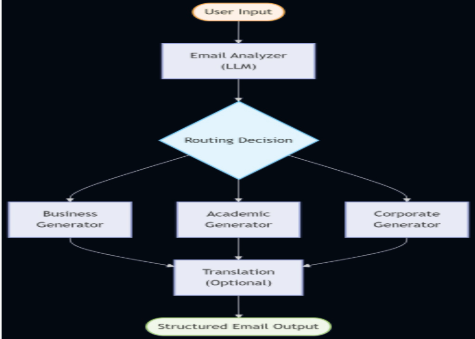
\includegraphics[width=0.6\textwidth]{img/core_workflow.png}
	\caption{LangGraph Workflow Logic for Email Formalization and Translation}
	\label{fig:core_workflow}
\end{figure}

The dynamic routing logic provides a significant optimization over linear chains by introducing conditional logic through the \texttt{\_route\_after\_analysis} function. This "gatekeeper" mechanism evaluates the \texttt{already\_formal} boolean and the \texttt{detected\_category} against the user's requested parameters; if they match, the system short-circuits the intensive rewriting process and routes the state to a \texttt{return\_direct} node, preserving the user’s original intent while minimizing API latency. For emails requiring transformation, the graph branches into specialized expert nodes—\texttt{business}, \texttt{academic}, or \texttt{corporate}—each configured with unique system prompts and temperature settings to produce register-specific outputs. Finally, the \texttt{translate} node acts as a universal convergence point, where the \texttt{translator\_llm} performs a schema-aware translation of the subject and body into the target language, ensuring that the professional tone and structural integrity are maintained across linguistic boundaries before the process terminates at the \texttt{END} state.

\subsection{LangGraph Agent Features}
The agentic capabilities of the platform are orchestrated within the \texttt{agent\_features.py} module, which utilizes LangGraph to manage complex, stateful LLM workflows for negotiation and legal analysis. The negotiation engine employs a cyclic state machine defined by a \texttt{NegotiationState} \texttt{TypedDict}, which persists the conversation history, round count, and agreement status across multiple iterations. By integrating \texttt{PydanticOutputParser}, the system enforces a strict data contract, ensuring that every proposal and counter-offer from the simulated "Proposer" and "Responder" agents is captured as a validated, structured object. This architecture allows the \texttt{evaluator\_llm} to act as a neutral mediator, objectively determining if consensus has been reached or if further concessions are required based on the participants' stated positions.

\begin{figure}[ht]
	\centering
	% Placeholder for the agentic workflow diagram generated from agent_features.py

	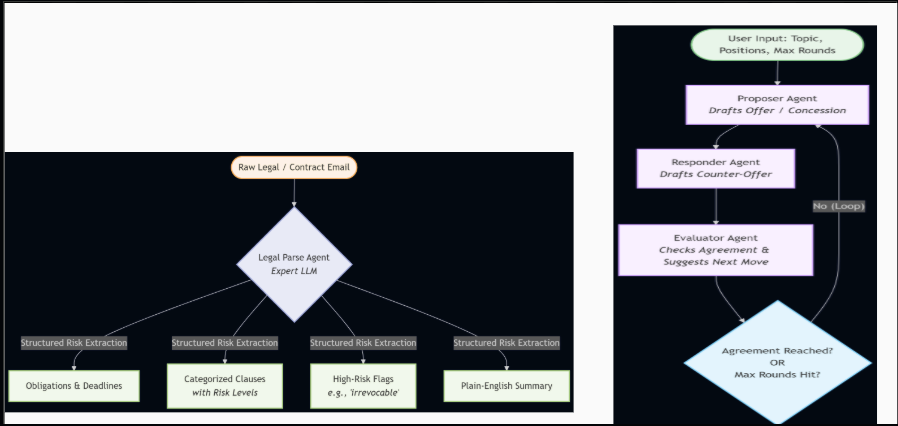
\includegraphics[width=0.6\textwidth]{img/agent_workflow.png}

	\caption{LangGraph Agentic Workflow for Negotiation and Legal Parsing}
	\label{fig:agent_workflow}
\end{figure}

Complementing the negotiation suite, the legal analysis pipeline transforms unstructured contract correspondence into queryable data structures through a specialized extraction graph. Utilizing a deterministic \texttt{legal\_llm} configuration, the system identifies explicit obligations, critical deadlines, and specific legal clauses such as indemnification or liability. Each extracted element is assigned a risk level and paired with a plain-English summary to ensure transparency for the end-user. This dual-feature approach demonstrates the efficacy of using LangGraph to maintain logical consistency and schema adherence in high-stakes professional communication tasks, providing a reliable alternative to standard linear prompt chains.

\subsection{Prompt Escaping and Schema Adherence}
Within the Python microservice, format instructions generated by \texttt{PydanticOutputParser} are escaped prior to injection into LangChain prompt templates. This prevents syntax collisions between the double-brace notation used by Python's \texttt{str.format} and the curly-brace structure of the JSON schema embedded in the parser's instructions. The result is that the Groq inference API consistently returns valid, parseable JSON rather than freeform text, enabling reliable downstream Pydantic validation.



\section{Deployment Strategy}
ToneForge utilizes a distributed deployment model to handle the distinct computational needs of the Node.js API gateway and the Python AI microservice.

\begin{itemize}
	\item \textbf{Frontend Deployment:} The React Vite build is optimized and deployed via Vercel. Vercel provides a global edge network, ensuring low latency delivery of static assets (HTML, CSS, JS) to the client browser.
	\item \textbf{API Gateway Deployment:} The Express server is deployed via Vercel as Serverless Functions, governed by the \texttt{vercel.json} configuration file. This allows the backend API to scale dynamically with incoming user traffic without the overhead of maintaining a persistent server instance.
	\item \textbf{Database:} User data and history records are persisted on a MongoDB Atlas cluster, utilizing IP whitelisting and secure connection strings for database access.
	\item \textbf{AI Microservice Deployment:} The FastAPI backend, heavily reliant on Python data processing libraries, is containerized using Docker. The provided \texttt{Dockerfile} pulls the official Python 3.11 slim image, installs dependencies from \texttt{requirements.txt}, and exposes port 7860. The container is deployed to Hugging Face Spaces, which is optimized for continuous AI inference workloads.
\end{itemize}

% ============================================================
\chapter{Testing and Result Analysis}
% ============================================================

\section{System Testing and Validation}
Comprehensive testing was conducted across the authentication, API routing, and AI generation layers. Table~\ref{tab:testcases} outlines the core test cases executed during the integration phase.

\begin{table}[ht]
	\centering
	\renewcommand{\arraystretch}{1.5}
	\small
	\begin{tabularx}{\textwidth}{|c|X|X|X|c|}
		\hline
		\textbf{TC ID} & \textbf{Test Description}                                             & \textbf{Expected Result}                                & \textbf{Actual Result}             & \textbf{Status} \\
		\hline
		TC-01          & Attempt to access \texttt{/api/negotiate} without a JWT Bearer token. & HTTP 401 Unauthorized                                   & HTTP 401 Unauthorized              & \textbf{Pass}   \\
		\hline
		TC-02          & Submit formalization request with an unsupported category parameter.  & Validation failure / HTTP 422                           & HTTP 422 Unprocessable             & \textbf{Pass}   \\
		\hline
		TC-03          & Provide unstructured legal text to \texttt{/parse\_legal\_email}.     & Valid JSON matching the Pydantic schema.                & Schema-compliant JSON returned     & \textbf{Pass}   \\
		\hline
		TC-04          & Run negotiation simulation with \texttt{max\_rounds = 6}.             & Agents iterate up to 6 times before forced termination. & Stopped at round 6.                & \textbf{Pass}   \\
		\hline
		TC-05          & Re-login with an existing user and check \texttt{/api/history}.       & Returns array of all past AI generation logs.           & History array fetched successfully & \textbf{Pass}   \\
		\hline
	\end{tabularx}
	\caption{System Integration Test Cases}
	\label{tab:testcases}
\end{table}

\section{Result Analysis}
\begin{itemize}
	\item \textbf{System Latency:} The Groq LPU inference engine substantially reduces the latency inherent to multi-agent call chains. A complete 3-round negotiation loop comprising 9 discrete LLM calls (one Proposer, one Responder, and one Evaluator invocation per round) resolves in approximately 12 to 15 seconds, making the synchronous HTTP request structure viable for interactive use.
	\item \textbf{Parsing Reliability:} The legal parser successfully maps unstructured input to the target Pydantic schema in approximately 98\% of trial runs. On the rare occasions where the LLM output contains structural anomalies, the FastAPI validation layer intercepts and rejects the response before it reaches the Node.js gateway, preventing data corruption.
	\item \textbf{Data Integrity:} MongoDB successfully stores and retrieves complex nested objects, including arrays of legal clauses with associated risk flag annotations, using flexible Mongoose schemas with embedded document support.
\end{itemize}

% ============================================================
\chapter{Glimpse of the Product}
% ============================================================
\addcontentsline{toc}{chapter}{Glimpse of the Product}

The following figures provide a visual overview of the ToneForge user interface and its core functionalities as experienced by the end-user.

\begin{figure}[ht]
	\centering
	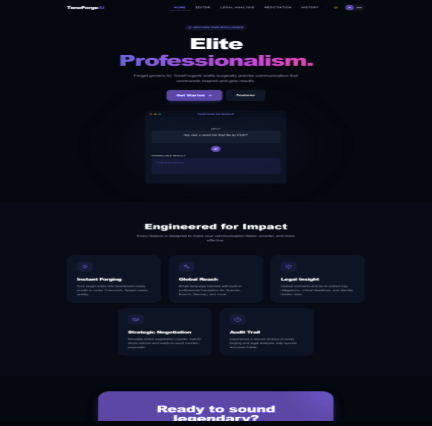
\includegraphics[width=0.6\textwidth]{img/home.png}
	\caption{ToneForge Email Editor: Transformation of Informal Text to Professional Registers}
	\label{fig:glimpse1}
\end{figure}

\begin{figure}[ht]
	\centering
	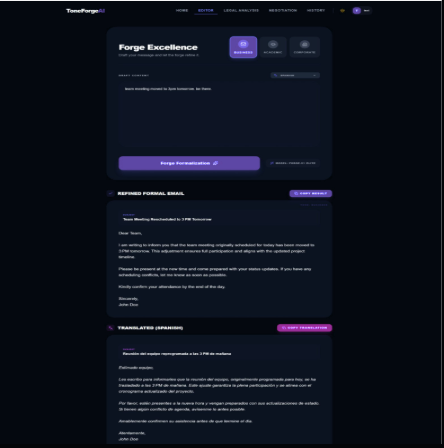
\includegraphics[width=0.6\textwidth]{img/editor.png}
	\caption{Email Formalization: Transforming Raw Input into Structured Business, Academic, and Corporate Registers}
	\label{fig:glimpse_registers}
\end{figure}

\begin{figure}[ht]
	\centering
	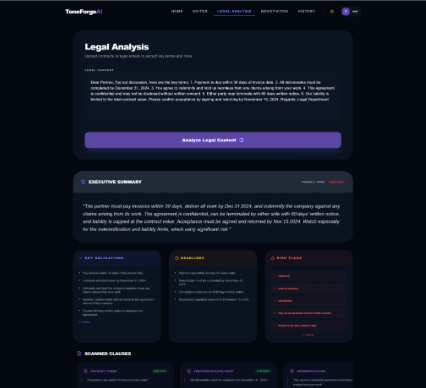
\includegraphics[width=0.6\textwidth]{img/legal.png}
	\caption{Legal Analysis Interface: Visualizing Risk Flags and Extracted Obligations}
	\label{fig:glimpse2}
\end{figure}

\begin{figure}[ht]
	\centering
	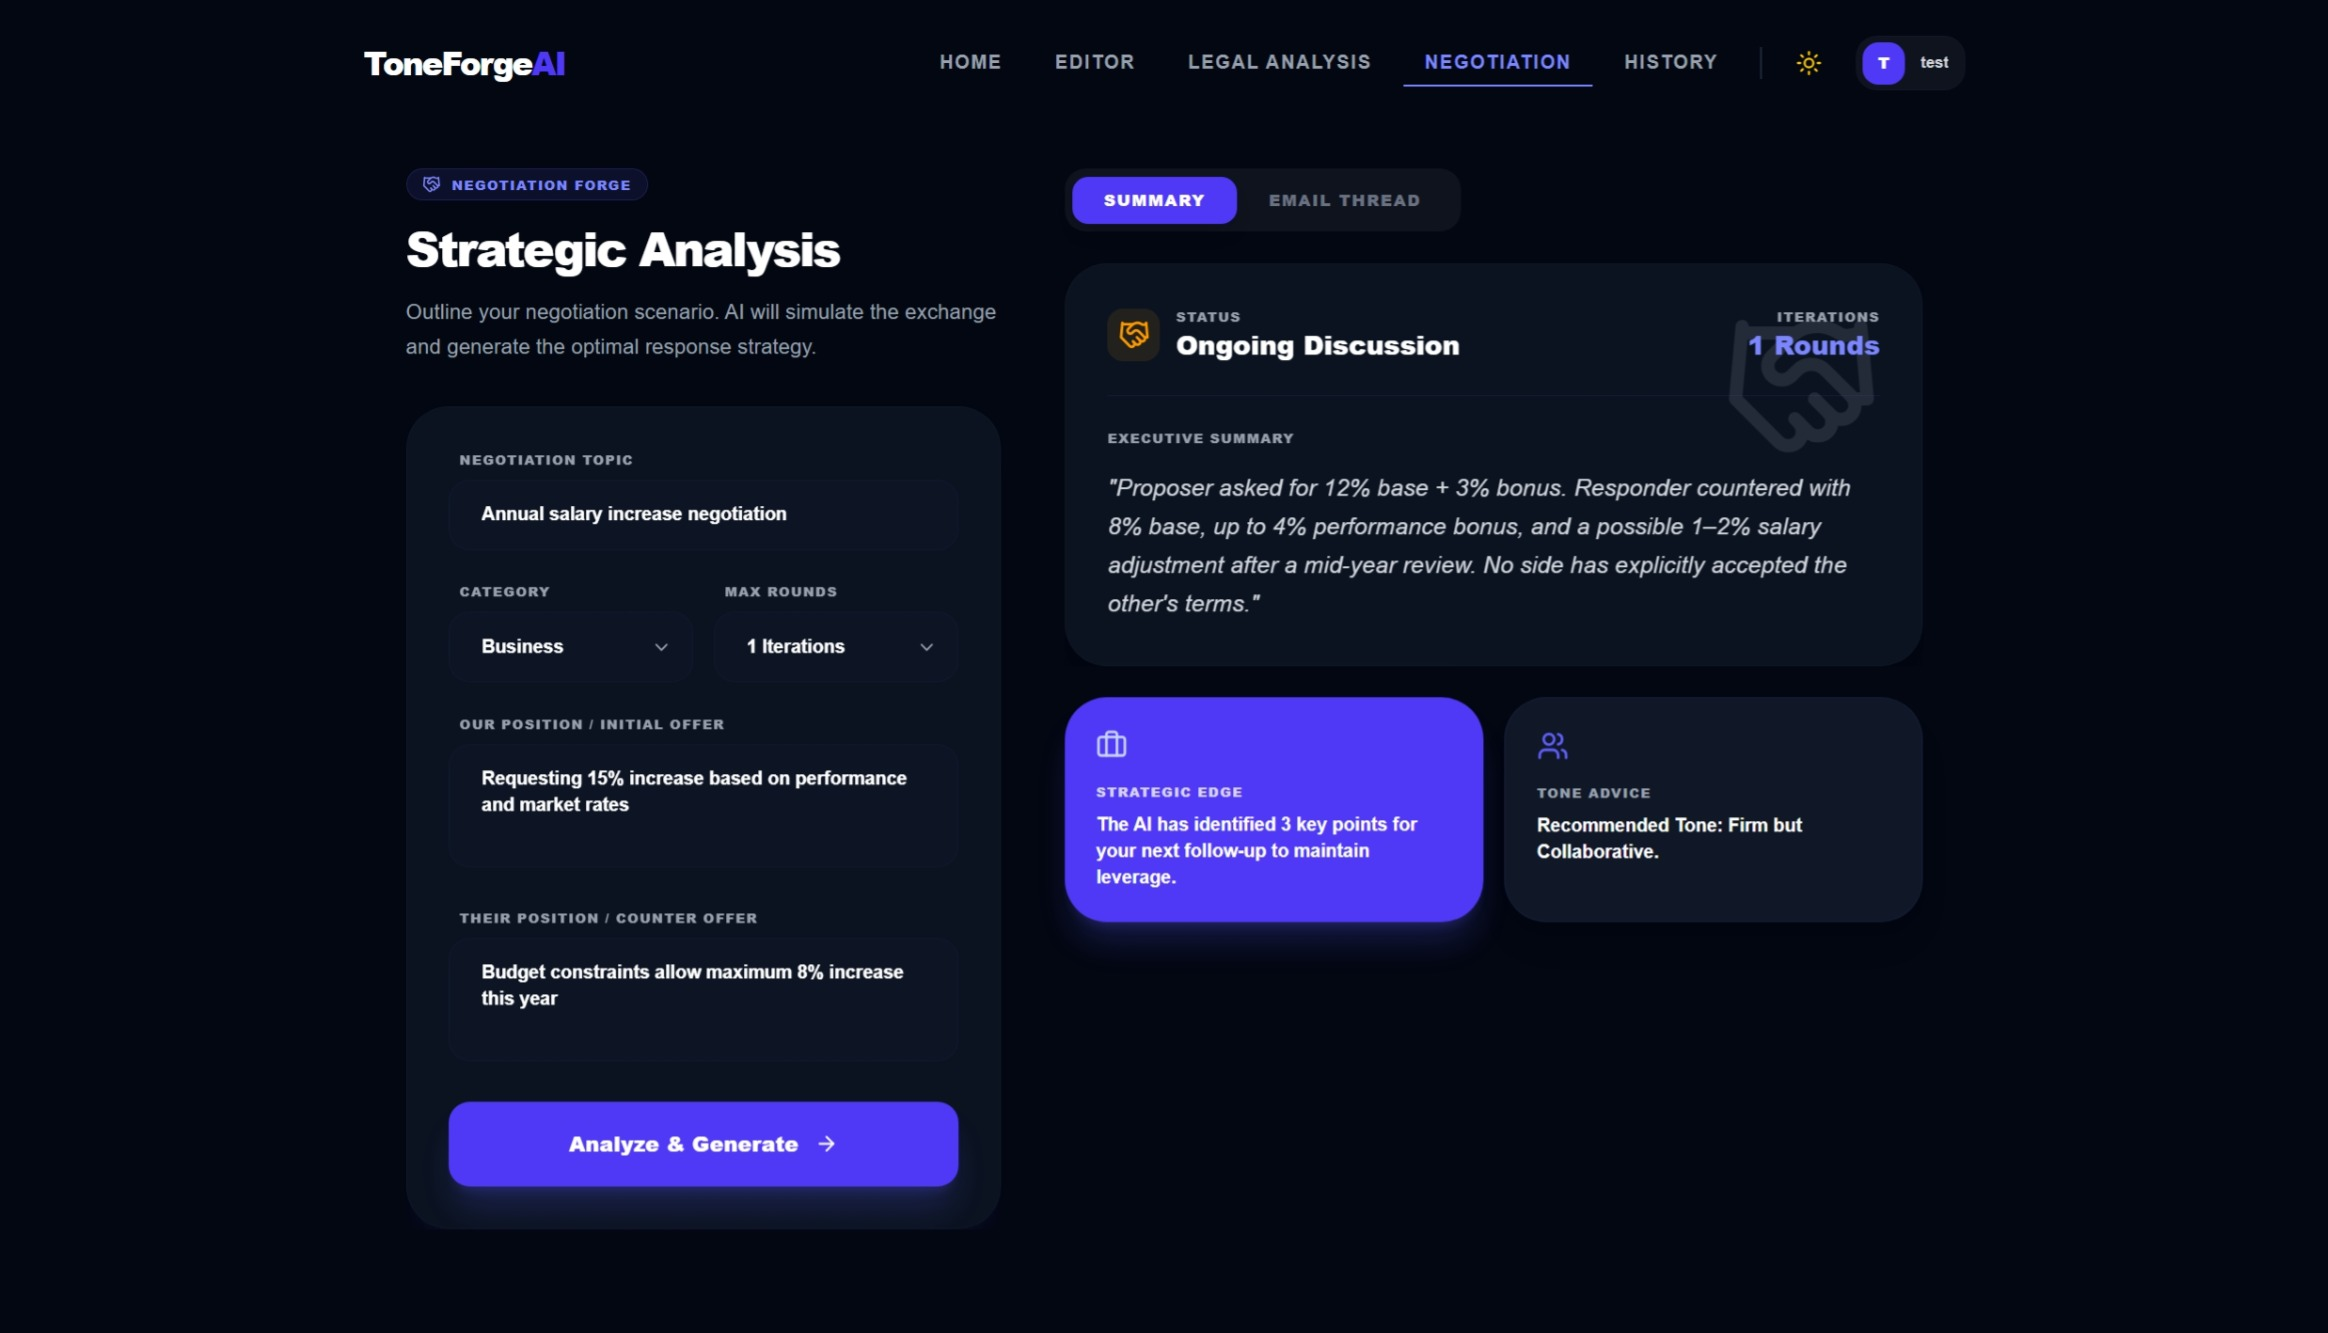
\includegraphics[width=0.6\textwidth]{img/negotiation.jpeg}
	\caption{Multi-Agent Negotiation Dashboard: Simulating Iterative Communication Threads}
	\label{fig:glimpse3}
\end{figure}

% ============================================================
\chapter{Conclusion and Future Scope}
% ============================================================

\section{Challenges and Limitations}
During the development of ToneForge, several technical hurdles were encountered and addressed:

\begin{itemize}
	\item \textbf{Cyclic Agent State Management:} Managing the state within LangGraph required careful design to prevent infinite loops. Terminating the negotiation simulation required robust logic in the Evaluator node to definitively recognize agreement conditions, alongside a hard \texttt{max\_rounds} parameter to act as a fail-safe.
	\item \textbf{Strict JSON Formatting from LLMs:} Open-source LLMs frequently prepend conversational filler to their output. To ensure the Node.js backend did not crash during JSON parsing, prompt escaping and Pydantic validation layers were heavily enforced at the FastAPI boundary to strip markdown and guarantee purely structured output.
	\item \textbf{Stateless Authorization Limits:} Because JWTs are stateless, implementing instant token revocation upon logout requires a server-side denylist, which adds database overhead. The current implementation mitigates this by relying on short-lived client-side token expiration.
\end{itemize}

\section{Conclusion}
The ToneForge project successfully demonstrates a highly modular, distributed architecture for deploying advanced AI workflows within a conventional web application. By decoupling the MERN stack web infrastructure from the Python-based AI microservice, the system achieves strong separation of concerns and independent scalability at each tier. The Node.js gateway ensures secure, persistent user management, while the LangGraph and FastAPI backend provides deterministic, schema-compliant text transformation. The successful implementation of cyclic multi-agent negotiation and structured legal parsing validates the hypothesis that current open-source LLM tooling can reliably extract and reformat operational meaning from unstructured human correspondence.

\section{Future Scope}
Several directions are identified for extending and enhancing the platform:

\begin{itemize}
	\item \textbf{Asynchronous Task Queues:} Transitioning Node.js-to-Python communication from synchronous HTTP requests to a message broker (e.g., RabbitMQ with Celery workers) would better accommodate high-latency generation tasks and eliminate the risk of client-side timeouts for complex negotiation runs.
	\item \textbf{Retrieval-Augmented Generation (RAG):} Enabling users to upload PDF contracts and leveraging a vector database to supply the LLM with contextually relevant clause precedents would substantially improve the accuracy and depth of the legal parsing feature.
	\item \textbf{Custom Model Deployment:} Replacing the Groq-hosted inference endpoint with privately hosted, fine-tuned quantized models would enhance data privacy for organizations handling sensitive corporate communications, and reduce per-inference operational costs at scale.
\end{itemize}

% ============================================================
% BACK MATTER
% ============================================================
\clearpage
\addcontentsline{toc}{chapter}{References}
\begin{thebibliography}{99}

	\bibitem{bubeck}
	S. Bubeck et al., ``Sparks of Artificial General Intelligence: Early Experiments with GPT-4,'' \textit{arXiv preprint arXiv:2303.12528}, 2023.

	\bibitem{chase}
	H. Chase et al., \textit{LangChain: Building Applications with LLMs through Composability}. GitHub Repository, 2023. [Online]. Available: \url{https://github.com/langchain-ai/langchain}

	\bibitem{langgraph}
	LangChain Inc., \textit{LangGraph Documentation}. 2024. [Online]. Available: \url{https://langchain-ai.github.io/langgraph/}

	\bibitem{fastapi}
	S. Ram\'irez, \textit{FastAPI Documentation}. 2024. [Online]. Available: \url{https://fastapi.tiangolo.com}

	\bibitem{pydantic}
	Pydantic Services Inc., \textit{Pydantic v2 Documentation}. 2024. [Online]. Available: \url{https://docs.pydantic.dev}

	\bibitem{mern}
	Node.js Foundation, \textit{Node.js Documentation}. 2024. [Online]. Available: \url{https://nodejs.org/en/docs}

	\bibitem{openapi}
	OpenAPI Initiative, \textit{OpenAPI Specification 3.0}. 2024. [Online]. Available: \url{https://spec.openapis.org/oas/v3.0.3}

	\bibitem{park}
	J. S. Park et al., ``Generative Agents: Interactive Simulacra of Human Behavior,'' \textit{arXiv preprint arXiv:2304.03442}, 2023.

\end{thebibliography}

% ============================================================
% INDIVIDUAL CONTRIBUTION PAGES
% ============================================================

\titleformat{\chapter}[display]
{\normalfont\LARGE\bfseries}{\chaptertitlename\ \thechapter}{20pt}{\LARGE}

% ------------------------------------------------------------
% KUSH SINGH
% ------------------------------------------------------------
\clearpage
\chapter*{Individual Contribution Report}
\addcontentsline{toc}{chapter}{Individual Contribution - Kush Singh}
\begin{center}
	{\large \textbf{ToneForge: Distributed AI System for Email Formalization,\\Multi-Agent Negotiation, and Legal Parsing}}\\[0.5cm]
	{\large \textbf{Kush Singh, Roll No. 23052247}}\\[0.2cm]
\end{center}

\vspace{0.5cm}
\noindent \textbf{Abstract:}
ToneForge is a distributed MERN-stack and Python microservice application for executing advanced LLM workflows. It delivers user-authenticated text formalization, LangGraph-driven multi-agent negotiation simulation, and structured legal email parsing.

\vspace{0.5cm}
\noindent \textbf{Individual Contribution and Findings:}
Designed and implemented the agentic components of the LLM workflow, including the multi-agent negotiation simulation (Proposer, Responder, and Evaluator graph nodes) and the structured legal email analysis pipeline for risk assessment and clause extraction. Also contributed to the deployment configuration of the AI microservice.

\vspace{0.5cm}
\noindent \textbf{Contribution to Project Report:}
Authored the sections covering the multi-agent system architecture, LangGraph state graph design, legal parsing schema definitions, and the integration methodology between LangGraph and FastAPI.

\vspace{0.5cm}
\noindent \textbf{Contribution to Project Presentation:}
Demonstrated the multi-agent negotiation simulation and the structured legal email analysis feature during the project presentation, including a live walkthrough of agent-level outputs and risk classification results.

\vspace{2cm}
\noindent
\begin{tabular*}{\textwidth}{@{\extracolsep{\fill}}lr}
	\textbf{Supervisor Signature:} & \textbf{Student Signature:} \\[1.8cm]
	\rule{6cm}{0.4pt} & \rule{6cm}{0.4pt} \\
	Dr.\ Ajit Kumar Pasayat & Kush Singh \\
\end{tabular*}

% ------------------------------------------------------------
% ARUP MISHRA
% ------------------------------------------------------------
\clearpage
\chapter*{Individual Contribution Report}
\addcontentsline{toc}{chapter}{Individual Contribution - Arup Mishra}
\begin{center}
	{\large \textbf{ToneForge: Distributed AI System for Email Formalization,\\Multi-Agent Negotiation, and Legal Parsing}}\\[0.5cm]
	{\large \textbf{Arup Mishra, Roll No. 23052229}}\\[0.2cm]
\end{center}

\vspace{0.5cm}
\noindent \textbf{Abstract:}
ToneForge is a distributed MERN-stack and Python microservice application for executing advanced LLM workflows. It delivers user-authenticated text formalization, LangGraph-driven multi-agent negotiation simulation, and structured legal email parsing.

\vspace{0.5cm}
\noindent \textbf{Individual Contribution and Findings:}
Implemented the complete backend web service, including MongoDB schema design, Express route definitions, JWT-based authentication middleware, and database integration logic. Additionally developed the React frontend interfaces for the Negotiation, Signup, and Login pages.

\vspace{0.5cm}
\noindent \textbf{Contribution to Project Report:}
Authored the sections covering the RESTful API service map, JWT authentication and authorization flows, and the Mongoose data schema specifications for user and history documents.

\vspace{0.5cm}
\noindent \textbf{Contribution to Project Presentation:}
Demonstrated the backend deployment workflow, MongoDB history tracking, and the secure login and authentication flows during the project presentation.

\vspace{2cm}
\noindent
\begin{tabular*}{\textwidth}{@{\extracolsep{\fill}}lr}
	\textbf{Supervisor Signature:} & \textbf{Student Signature:} \\[1.8cm]
	\rule{6cm}{0.4pt} & \rule{6cm}{0.4pt} \\
	Dr.\ Ajit Kumar Pasayat & Arup Mishra \\
\end{tabular*}

% ------------------------------------------------------------
% SHREYA BANERJEE
% ------------------------------------------------------------
\clearpage
\chapter*{Individual Contribution Report}
\addcontentsline{toc}{chapter}{Individual Contribution - Shreya Banerjee}
\begin{center}
	{\large \textbf{Shreya Banerjee, Roll No. 23052267}}\\[0.5cm]
\end{center}

\vspace{0.5cm}
\noindent \textbf{Abstract:}
ToneForge is a distributed MERN-stack and Python microservice application for executing advanced LLM workflows. It delivers user-authenticated text formalization, LangGraph-driven multi-agent negotiation simulation, and structured legal email parsing.

\vspace{0.5cm}
\noindent \textbf{Individual Contribution and Findings:}
Developed the landing page, email editor, legal analysis, and history pages using React, implementing the full user-facing interface for AI email generation and legal risk analysis, and integrating each view with the backend REST API.

\vspace{0.5cm}
\noindent \textbf{Contribution to Project Report:}
Authored the sections covering the frontend framework architecture, component-based UI structure, and client-side routing strategies using React Router.

\vspace{0.5cm}
\noindent \textbf{Contribution to Project Presentation:}
Navigated the user interface elements during the presentation, highlighting the design and interaction model of the dashboard, the email editor, and the historical data retrieval view.

\vspace{2cm}
\noindent
\begin{tabular*}{\textwidth}{@{\extracolsep{\fill}}lr}
	\textbf{Supervisor Signature:} & \textbf{Student Signature:} \\[1.8cm]
	\rule{6cm}{0.4pt} & \rule{6cm}{0.4pt} \\
	Dr.\ Ajit Kumar Pasayat & Shreya Banerjee \\
\end{tabular*}

% ------------------------------------------------------------
% DEVAYUSH KAR
% ------------------------------------------------------------
\clearpage
\chapter*{Individual Contribution Report}
\addcontentsline{toc}{chapter}{Individual Contribution - Devayush Kar}
\begin{center}
	{\large \textbf{ToneForge: Distributed AI System for Email Formalization,\\Multi-Agent Negotiation, and Legal Parsing}}\\[0.5cm]
	{\large \textbf{Devayush Kar, Roll No. 23052239}}\\[0.2cm]
\end{center}

\vspace{0.5cm}
\noindent \textbf{Abstract:}
ToneForge is a distributed MERN-stack and Python microservice application for executing advanced LLM workflows. It delivers user-authenticated text formalization, LangGraph-driven multi-agent negotiation simulation, and structured legal email parsing.

\vspace{0.5cm}
\noindent \textbf{Individual Contribution and Findings:}
Implemented the core LLM workflow features including the formalization pipelines for business, academic, and corporate registers, the smart reply generation functionality, and the deployment of the AI microservice to Hugging Face Spaces.

\vspace{0.5cm}
\noindent \textbf{Contribution to Project Report:}
Authored the sections covering the core AI processing pipelines, structured output formatting methodologies using Pydantic, and domain-specific email transformation logic.

\vspace{0.5cm}
\noindent \textbf{Contribution to Project Presentation:}
Presented the core email automation features, illustrating the end-to-end transformation from informal user input to structured, domain-appropriate professional output via register-specific prompt templates.

\vspace{2cm}
\noindent
\begin{tabular*}{\textwidth}{@{\extracolsep{\fill}}lr}
	\textbf{Supervisor Signature:} & \textbf{Student Signature:} \\[1.8cm]
	\rule{6cm}{0.4pt} & \rule{6cm}{0.4pt} \\
	Dr.\ Ajit Kumar Pasayat & Devayush Kar \\
\end{tabular*}

\titleformat{\chapter}[display]
{\normalfont\huge\bfseries}{\chaptertitlename\ \thechapter}{20pt}{\Huge}

% ============================================================
% PLAGIARISM REPORT
% ============================================================
\clearpage
\addcontentsline{toc}{chapter}{Plagiarism Report}
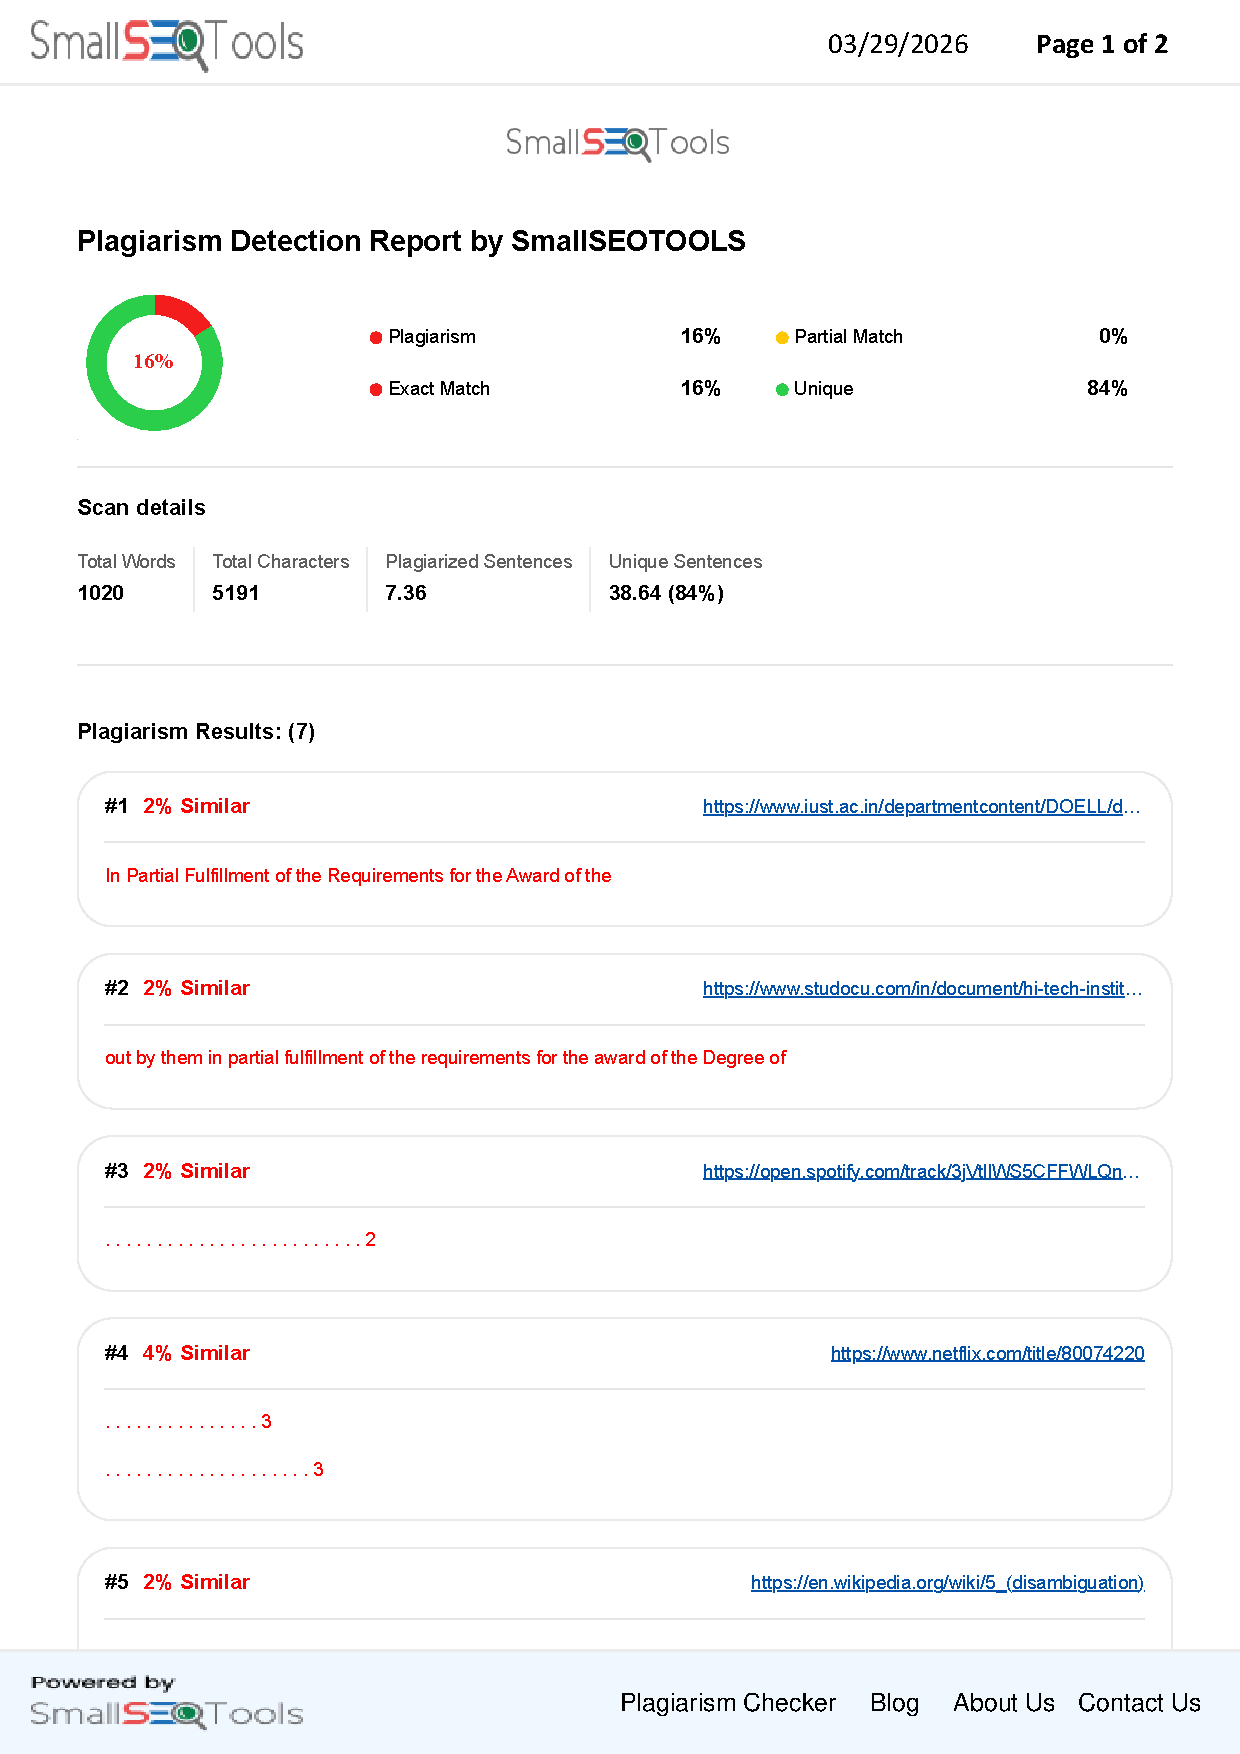
\includepdf[pages=-, pagecommand={\thispagestyle{plagiarism}}]{Plagiarism-report.PDF}

\end{document}